\section{Introduction}

In this chapter we develop a new model of frequency spectra, amenable to distributed reconstruction. We then apply the algorithm from chapter \ref{chap:dist-opt}, combined with this model, to perform spectrum sensing.

Compressive sensing makes the assumption that the signal being sensed is sparse, however we cannot always guarantee that the frequency spectrum will always be sparse: for example, should TVWS become widely utilised, the spectra will not be sparse. However, even for highly occupied spectra, the gradient of the spectrum will be sparse. This is because that TVWS spectra will feature bands with a flat power spectrum when occupied - or occupied bands will be well approximated by rectangular bands. Thus the PSD will feature abrupt changes in its gradient during transitions between occupied and unoccupied bands. This has previously been exploited by \cite{tian2006wavelet}. 

Reconstructing the spectrum from compressive measurements could take place at a fusion centre, but such communications are expensive. It is more efficient therefore to design distributed algorithms where CRs communicate with their neighbours to reach consensus on the reconstruction, given each nodes' private data. However, regularising the reconstruction process would require global co-ordination if Total Variation (the \(l_1\) norm of the gradient of the signal) regularisation was chosen, as.

In this chapter we propose a different model for sensing the gradient of the frequency spectrum to \cite{tian2006wavelet} - a model which doesn't require Total Variation regularisation of the objective function. 

The structure of the chapter is as follows: in section \ref{sec:sig-model} we introduce the signal model, in \ref{Time-Frequency Model} we introduce the sensing model, and in section \ref{sec:results} we show some results of the reconstruction quality of this model. 

\section{Signal Model}\label{sec:sig-model}

Not all signals are sparse in an orthogonal basis: for example, many images are sparse in an over-complete dictionary (set of bases). In particular, frequency spectra for TVWS may no longer be sparse once opportunistic radios begin operating in these frequency bands. 

Instead we aim to reconstruct the gradient of the spectrum, as we assume that transitions are constant within a band. Consider the basis defined by the function:

\begin{definition}[Heaviside Basis]
\begin{equation}
l_i\left(x\right) =
\begin{cases}
1 & \text{if } x \leq i \\
0 & \text{ otherwise } 
\end{cases}
\label{basis}
\end{equation}

That is, \(l_i\) is a left-hand step function. 

The basis (\ref{basis}) can be expressed as a matrix in \(\re^{n \times n}\) as, where basis vectors are written as rown of \(L_n\):

\begin{equation}
L_n = \begin{pmatrix}
 1 & 0 & 0 & 0  & 0 \ldots 0 \\
  1 & 1 & 0 & 0  & 0 \ldots 0\\
     1 & 1 & 1 & 0  & 0 \ldots0  \\
    \ldots  \\
     1 & 1 & 1 & 1  & 1 \ldots 1 
\end{pmatrix}
\end{equation}
In gneral we write \(L_m\) for an \(m \times m\) matrix of this form.
\end{definition}

\begin{lemma}
By direct computation, this inverse of \(L_n\) is:

\begin{equation}
D_n = \begin{pmatrix}
 1 & 0 & 0 & 0  & 0 \ldots 0 \\
  -1 & 1 & 0 & 0  & 0 \ldots 0\\
     0 & -1 & 0 & 0  & 0 \ldots0  \\
    \ldots  \\
     0 & 0 & 0 & 0  \ldots -1 & 1
\end{pmatrix}
\end{equation}
In gneral we write \(D_m = L_m^{-1}\) for an \(m \times m\) matrix of this form.
\end{lemma}

\begin{definition}
We model our PSD signal \(g\) as a linear combination of the basis functions (\ref{basis}):

\begin{equation}
g\left(x\right) = \sum_i q_i l_i\left(x\right) = L^Tq
\label{basis-expansion}
\end{equation}

where \(q = (q_1, \ldots, q_n\) are the coefficients in this basis expansion, and \(l_i\) are the rows of \(L\). Note that as defined, \(g\) is a column vector.
\end{definition}

\begin{definition}
We can define a matrix representation for the set of basis vectors \(l_i\), by taking all inner products between all pairs of basis vectors:

\begin{equation}
F_{n, ij} = \langle l_i, l_j \rangle
\end{equation}

This matrix has the representation:

\begin{equation}
F_{ij} = \min(i,j)
\end{equation}

An example of such a matrix is:

\begin{equation}
F_n= \begin{pmatrix}
 1 & 1 & 1 & 1  & 1 \\
  1 & 2 & 2 & 2  & 2\\
     1 & 2 & 3 & 3  & 3  \\
    1 & 2 & 3 & 4  & 4  \\
     1 & 2 & 3 & 4  & 5 
\end{pmatrix}
\label{def:Fmtx}
\end{equation}
\end{definition}

\begin{theorem}
This matrix is invertible since:

\begin{equation}
\det(F_n) = 1
\end{equation}
\end{theorem}
\begin{proof}
Consider the matrix \(F_n\). Subtract the \(n-1\)th column from the \(n\)th. We obtain a matrix with \(0\) on the final column except the entry \(F_n(n,n) = 1\). Since the top \((n-1) \times (n-1)\) is \(F_{n-1}\) we find that 

\begin{equation}
\det(F_n) = 1 \times \det(F_{n-1})
\end{equation} 

By recursion and \(\det(F_1) = 1\) we have \(\det(F_n) = 1\).

\end{proof}

This matrix can be factorised as \(F = LL^T\).

From this it follows that

\begin{equation}
F_n^{-1} = \begin{pmatrix}
 2 & -1 & 0 & 0  & 0 \ldots 0 \\
  -1 & 2 & -1 & 0  & 0 \ldots 0\\
     0 & -1 & 2 & -1  & 0 \ldots0  \\
    \ldots  \\
     0 & 0 & 0 & 0  \ldots -1 & 1 
\end{pmatrix} = D_n^TD_n
\end{equation}

To find the \(q_i\), we correlate (take the inner product of) the signal against the basis \eqref{basis}.

\begin{definition}[Inner Product]
We define the inner product between two vectors as follows:

\begin{equation}
\langle u, v \rangle = u^T v = \sum_i u_i v_i
\end{equation}	
where \(u_i, v_i\) are the components of the vectors \(u,v\) in the \(i^{th}\) direction with respect to some orthonromal basis vectors \(e_i\).

In general, for vectors which are not orthogonal, for example:

\begin{equation}
g = \sum_i a_i l_i\left(x\right)
\end{equation}

\begin{equation}
h = \sum_i b_i l_i\left(x\right)
\end{equation}

Then, the inner product can be expressed as:

\begin{equation}
\langle g, g \rangle = a^TL^TL b = a^T F b
\end{equation}	

\end{definition}

\begin{definition}[Cumulative Sum]
We can express the inner product between the signal \(g\) and the set of basis vectors as:

\begin{equation}
h_j = \langle g, l_j \rangle
\end{equation}

this is a useful quantity, as it is the cumulitive sum of the signal \(g\):

\begin{align}
h_j &= \langle g, l_j \rangle \\
&= \sum_x g\left(x\right) l_j\left(x\right) \\
&= \sum_x \sum_i a_i l_i\left(x\right) l_j\left(x\right) \\
&= \sum_i a_i \sum_x l_i\left(x\right) l_j\left(x\right)
&= a_i \langle l_i, l_j\rangle \\
\end{align}

In matrix language \(h = F q^T\). This is the inner product between the signal \(g\) and the basis functions \(l_i\).
\end{definition}


\begin{proposition}
We can recover the coefficients \(q\) from \(g\) easily since:
\begin{equation}
D_n^Tg = q
\end{equation}
\label{def:a}
\end{proposition}
\begin{proof}

\begin{align}
D_n^Tg &= D_n^T L_n^T q \\
&= \left(L_nD_n\right)^Tq \\
&= q
\end{align}

as \(L_nD_n = I_n\).

\end{proof}

\begin{example}[Single Rectangle]
Consider a signal \(g\left(x\right) \in \re^n\) which is 

\begin{equation}
g\left(x\right) =
\begin{cases}
1 & \text{if } \frac{n}{4} \leq x < \frac{3n}{4} \\
0 & \text{ otherwise } 
\end{cases}
\end{equation}

in the basis defined by \eqref{basis}, this function can be expressed as:

\begin{equation}
g\left(x\right) = L_n^Tq
\end{equation}

with 
\begin{equation}
q_i =
\begin{cases}
-1 & \text{if } i = \frac{n}{4} \\
1 & \text{if } i = \frac{3n}{4} \\
0 & \text{ otherwise } \\
\end{cases}
\end{equation}

\end{example}

Given a set of compressive measurements we can create an estimate of \(g\), by using procedure \ref{alg:single-slot}.

\begin{figure}
\begin{algorithmic}[1]
 %\SetAlgoLined % For previous releases [?]
 \Procedure{Estimate Occupancy}{$y$, $A$, $k$}
 \State{\textbf{Inputs}: A set compressive measurements \(y\), a measurement matrix \(A\), and an integer \(k\)}
 \State{\textbf{Returns}: \(\hat{g}\), an estimate of the occupancy of a frequency spectrum.}
 \\
Calculate \(g=A^ty\)
 \\
Choose a set of indices using procedure Index Pursuit
\\
 Between the indices of \(g\) take the average.
 \\
   	For each piece between the \(k\) changepoints, do a t-test to determine whether the signal is noise, or a transmission.
   	\EndProcedure
\end{algorithmic}
 \caption{Procedure for estimating occupancy of frequency spectra}
 \label{alg:single-slot}
\end{figure}

\begin{figure}
\begin{algorithmic}[1]
 %\SetAlgoLined % For previous releases [?]
 \Procedure{Index Pursuit}{}
 \State{\textbf{Inputs}: \(g=A^t y\), \(L\), \(F^{-1}\), \(k\)}
 \State{\textbf{Returns}: A set \({j}_{i=1}^k\) of indices}
 \\
 Set \(z = A^ty\), \(\mathrm{inds} = \varnothing \)
 \\ For \(i=1:k\):
 \\ Calculate \(u = Lz\), and \(\alpha = F^{-1}u\)
 \\ Find \(\max_i|\alpha|\)
 \\ Set \(z = z - \alpha_i e_i\)
 \\ Set \(\mathrm{inds} = \mathrm{inds}+i\)
 \EndProcedure
\end{algorithmic}
 \caption{Index pursuit for estimating changepoints in the signal \(A^ty\)}
 \label{alg:index_pursuit}
\end{figure}

\begin{figure}[h]
\centering
\includegraphics[height = 7.3 cm]{g.jpg}
\caption{}
\label{fig:rectangle}
\end{figure}

We now describe the procedure \ref{alg:single-slot}, in more detail. Given a set of compressive measurements: 

\begin{equation}
y = Ag = AL_n q^T
\end{equation}
\\
where \(A \in \re^{m \times n} \), \(A_{ij} \sim \mathcal{N}\left(0,1/m\right)\).
\\
We then compute 
\begin{equation}
\langle y, Al_i\rangle = q_j  l_j^TA^tAl_j \sim \frac{q_j}{m} \langle l_j, l_i \rangle
\label{key-step}
\end{equation}
for the set of basis vectors \(l_1 \ldots l_n\) i.e. the estimator from the previous section, corresponding to this set of basis functions \eqref{eq: compressive-estimator}. 

\begin{remark}
This is the key step in this procedure. The relation 

\begin{equation}
\langle y, Al_i\rangle = q_j  l_j^TA^tAl_j \sim \frac{q_j}{m} \langle l_j, l_i \rangle
\end{equation}

is valid because of the RIP \eqref{def:RIP} from chapter \ref{chap:cs}. We are using the fact that the matrix \(A^TA\) is \(\delta\)-close to an isometry (where \(\delta\) is the RIP constant of \(A\), along with the result of theorem \eqref{thm:wishart-mean}, to estimate the vector \(h\).

\end{remark}
We then form the vector 

\begin{equation}
\hat{h} = m \sum_i \langle y, Al_i\rangle l_j \sim h
\label{ss-estimator}
\end{equation}\textit{•}

Again, this relation (\(\sim\)) is based on the same reasoning as the previous equation \eqref{key-step}.

An example can be seen in figure \ref{fig:hhat}, for a matrix \(A \in \re^{200 \times 300}.\)

\begin{figure}[h]
\centering
\includegraphics[height = 7.3 cm]{hhat.jpg}
\caption{}
\label{fig:hhat}
\caption{An example of the estimate \(\hat{h}\) for a single rectange signal (in red) compared to the true cumultivie vector \(h\) (in blue). Note how the estimate tracks the true signal, with little deviation.}
\end{figure}

\section{Time-Frequency Model}
In this section we extend the model from section \ref{sec:freq-model}, to jointly estimate a collection of signals sensed over time. 

In this case, we have a series frequency spectra \(\in \re^n\), sensed at \(T\) time instants. We extend the model, again in the same basis:


\begin{equation}
l_{i,t}\left(x, \tau\right) = \mathbb{I}\left(t \leq \tau \right)\mathbb{I}\left(x \leq i\right)
\label{time-freq basis}
\end{equation}

We can express these basis functions in terms of the basis functions \eqref{basis}, and similarly defined basis functions over time:

\begin{equation}
l_t\left(\tau\right) =
\begin{cases}
1 & \text{if } t \leq \tau \\
0 & \text{ otherwise } 
\end{cases}
\label{time-basis}
\end{equation}

That is, \(l_t\) is again a left-hand step function. 

\begin{proposition}
\begin{equation}
l_{i,t}\left(x, \tau\right) = l_i\left(x\right) \kronecker l_t\left(\tau\right)
\end{equation}
\begin{proof}
Consider a fixed frequency, w.l.o.g \(i=1\). Then 
\begin{equation}
l_{1,t}\left(x, \tau\right) = \mathbb{I}\left(x \leq 1\right)\mathbb{I}\left(t \leq \tau \right)
\end{equation}
There are \(T\) possible vectors, each of length \(n\), for this combination of \(\left(i,t\right)\). Therefore \(l_{1,t}\in \re^{1\times nT} \). As there are \(n\) possible frequency vectors, one for each fixed frequency basis function, we have \(n\times nT\) vectors. By symmetry of time and frequency, the same argument applies for a fixed time, and we have \(T\), \(1\times nT\) basis vectors in total, one for each fixed time instant. Therefore the joint time-frequency basis is in \(\re^{nT \times nT}\). As time and frequency are orthogonal in this representation, the proposition follows.
\end{proof}
\end{proposition}

Thus this basis can be represented with the following matrix:

\begin{equation}
L = L_T \kronecker L_n
\label{def:time-freq matrix}
\end{equation}

where \(L_k\) is the matrix \eqref{lower-L} of size \(k \times k\). From \eqref{def:time-freq matrix}, it follows that:

\begin{equation}
D = L^{-1} = L_T^{-1} \kronecker L_n^{-1} = D_T \kronecker D_n
\end{equation}

where \(D_k\) is the same as \eqref{inv-L}, and that:

\begin{align}
F &= LL^T \\
&= \left(L_n \kronecker L_T\right)\left(L_n \kronecker L_T\right)^T\\
&=L_TL_T^T \kronecker L_nL_n^T \\
&= F_T \kronecker F_n
\end{align}

where \(F_k\) is defined as in \eqref{def:Fmtx}.

We sense the frequency spectrum at \(T\) instants, collecting signals \(g_1, \ldots g_\tau\). 

\begin{definition}
We define
\begin{equation}
G = \left[g_1, \ldots, g_\tau \right]
\end{equation}
and
\begin{equation}
g = \mathrm{vec}\left(G\right) = \dottedcolumn{3}{g_1}{g_\tau}
\end{equation}
\end{definition}

we also define:

\begin{definition}
\begin{equation}
a = \mathrm{vec}\left(a_t\right) = \sum_{t=1}^T e_t \kronecker a_t
\end{equation}
\end{definition}

These definitions are related by the formula:

\begin{equation}
g = L^Ta = \left(L_T^T \kronecker L_n^T\right)a
\end{equation}

We can find an expression for \(a\) by taking the inner product of \(g\) with \(l_{j,s}\):

\begin{align*}
h &= \langle g, l_{j,s}\left(x, \tau\right)\rangle \\
&= \sum_{i,t} g(x,\tau) \langle l_{i,t}, l_{j,s} \rangle \\
&= Fa
\end{align*}

where we have defined \(F = \left(F_T \kronecker F_n\right)\).

The measurements in this model can be written as

\begin{equation}
y_T = A_Tg
\end{equation}

with 

\begin{equation}
A_T = I_T \kronecker A
\end{equation}

and \(A \sim N(0, 1/m)\).

We consider the case where \(g_t = g\) for each time slot (i.e. the signal is unchanging). 

\begin{proposition}
We can write the \(i^{th}\) column of the matrix \(L_k\) as, for \(k \leq j\):

\begin{equation}
L_k^T e_i = \sum_{j=1}^i e_j
\end{equation}

where \(e_j\) is the \(j^{th}\) canonical basis vector in \(\re^k\), with has a \(1\) in position \(j\) and is zeros everywhere else.

\begin{proof}
The \(i^{th}\) column of \(L_k\) will have \(i\) ones, and \(k-i\) zeros. It can be written in terms of the canonical basis \(e_j\), simply as sum up to the last \(1\) in position \(i\).
\end{proof}

\end{proposition}

In this case, we can write \(g\) as:

\begin{align*}
g = L^T a &= \left(L_T^T \kronecker L_n^T\right)\left(\sum_{t=1}^T e_t \kronecker a_t\right) \\
&= \sum_{t=1}^T L_T^T e_j \kronecker L_n^Ta_t \\
&= \sum_{t=1}^T \left(\sum_{j=1}^n e_j \right) \kronecker L_n^T a_t \\
&= \sum_{j=1}^T e_j \kronecker \sum_{t=j}^T L_n^T a_t \\
&= \sum_{j=1}^T e_j \kronecker b_j
\end{align*}

where we define \(b_j = \sum_{t=j}^T L_n^T a_t\). We can now write

\begin{align*}
y_T = A_Tg &= \left(I_T \kronecker A \right) \left(\sum_{j=1}^T e_i \kronecker b_j\right)\\
&= \sum_{j=1}^T e_j \kronecker Ab_j
\end{align*}

\begin{example}
Now consider the case where all the \(a_t\) are identical. In this case:

\begin{equation}
\twopartdef{a_T = a}{t=T}{a_t = 0}{t < T}
\end{equation}

so

\begin{equation}
b_j = \sum_{t=j}^T L_n^T a_t = L_n^T a = b
\end{equation}

Then

\begin{equation}
y_T = \left( \sum_{j=1}^T \right) \kronecker Ab = 1_T \kronecker Ab
\end{equation}
\end{example}

Let the \(s^{th}\) column of \(L_T^T\) be denoted by \(B_s\), then

\begin{align*}
\left(L_T^T\right)^{-1}B_s = D_T^T B_s = e_s
\end{align*}

As before, we form the estimator

\begin{align*}
\hat{h}_T = \sum_{i,t} \langle y_T, A_T l_{i,t} \rangle l_{i,t} \sim \frac{1}{mT} Fa
\end{align*}

Consider 

\begin{align*}
\langle y_T, A_T l_{i,t} \rangle &= \langle A_T^T y_T,l_{i,t} \rangle \\
&= \langle \left(I_T \kronecker A^T\right)\left(\sum_{j=1}^T e_j \kronecker Ab_j\right), \left(l_t \kronecker l_i\right)\rangle \\
&= \langle \sum_{j=1}^T e_j \kronecker A^TAb_j, \left(l_t \kronecker l_i\right)\rangle \\
&= \sum_{j=1}^T e_j^T l_t \kronecker b_j^TA^TAl_i \\
&\sim \frac{1}{m}\sum_{j=1}^T e_j^T l_t \kronecker b_j^Tl_i\\
&\stackrel{?}{=} \frac{1}{m}\sum_{j=1}^T j \kronecker F_n a
\end{align*}

where we used the expectation of a Wishart matrix between the \(5^{th}\) and \(6^{th}\) lines.

\begin{definition}[Period-change vector]
Let
\begin{equation}
B = D \kronecker I_T
\end{equation}

then we define 

\begin{equation}
z = By
\end{equation}
\label{period vector}

This vector, identifies consecutive time slots in which the signal \(g\) is constant (i.e. does not change between sensing instants). As example, consider the following 5-slot signal:

\begin{figure}[h]
\centering
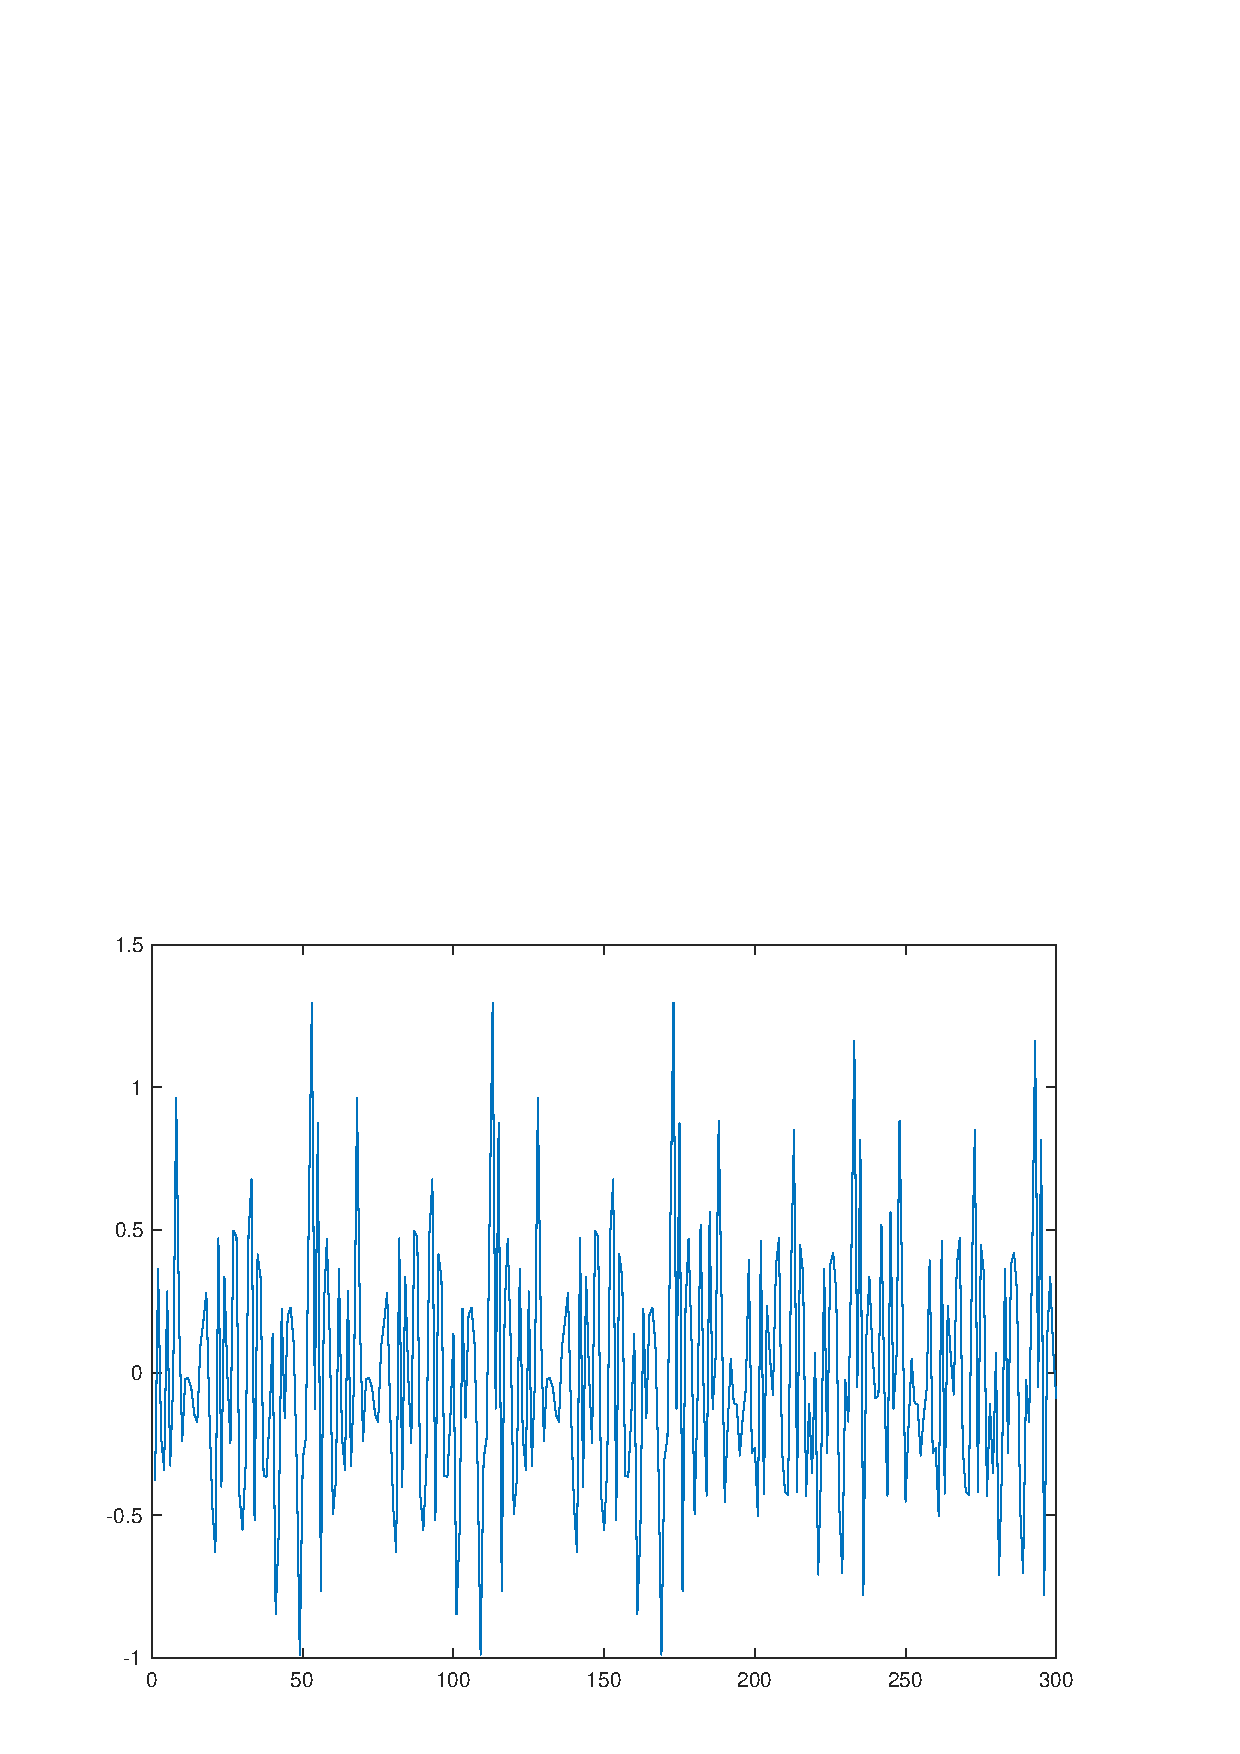
\includegraphics[height = 7.3 cm]{gt.jpg}
\caption{Example multiple time-slot signal}
\label{fig:gt}
\end{figure}

Whilst the compressive measurements of this signal are not revealing:

\begin{figure}[h]
\centering
\includegraphics[height = 7.3 cm]{gt-compressed.jpg}
\caption{Compressive Measurements of the previous signal \ref{gt}}
\label{fig:ygt}
\end{figure}

The period change vector clearly identiies the periods where the original signal changes:

\begin{figure}[h]
\centering
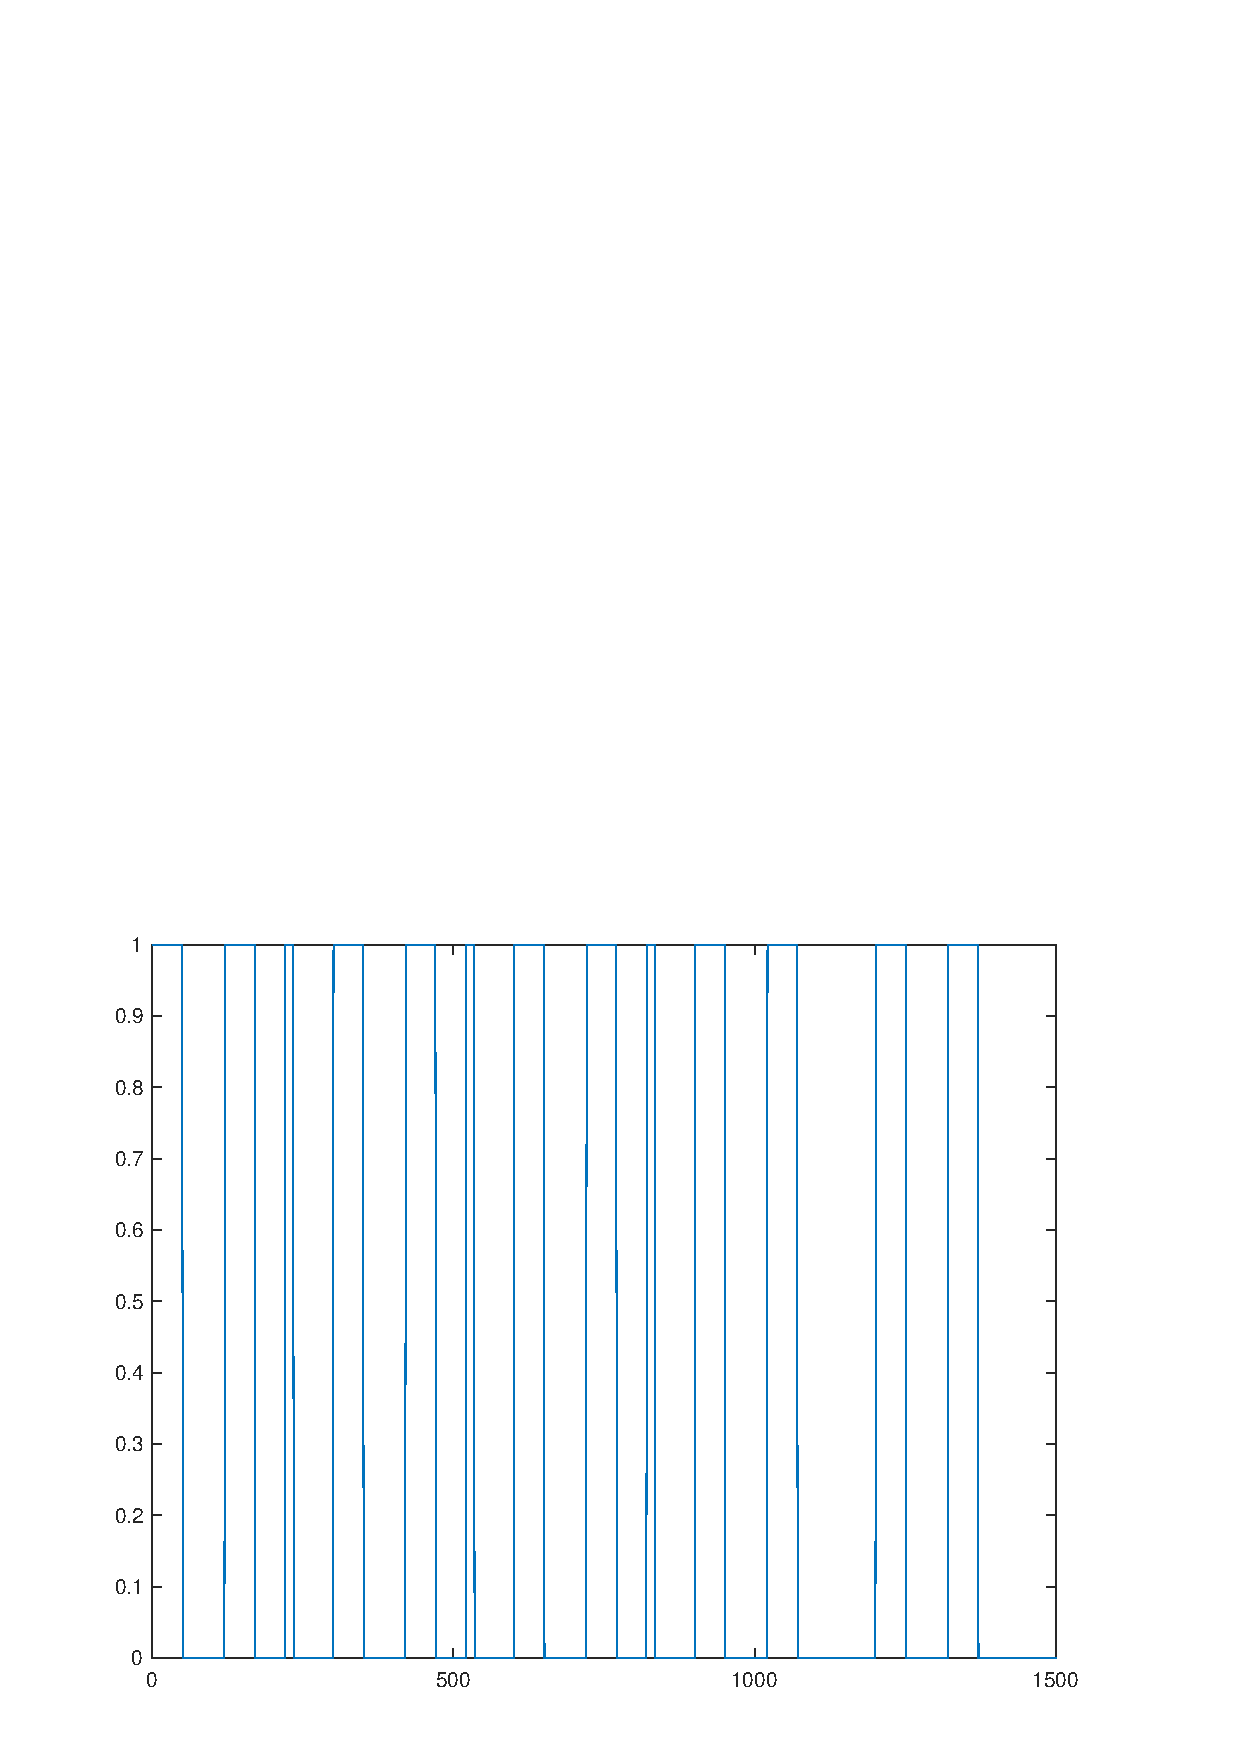
\includegraphics[height = 7.3 cm]{z-vec.jpg}
\caption{Period-change vector for the signal \ref{gt}}
\label{fig:period-vec}
\end{figure}

\end{definition}

We can use this vector to estimate a multiple time-slot signal. We use the following algorithm:

\begin{figure}
\begin{algorithmic}[1]
 %\SetAlgoLined % For previous releases [?]
 \Procedure{Estimate Occupancy Multiple Slot}{$y$, $A$, $k$}
 \State{A set compressive measurements \(y_T\), a measurement matrix \(A_T\), and an integer \(k\)}
 \State{\textbf{Returns}A estimate of the occupancy of a frequency spectrum, along multiple time slots.}
 \\
Compute \(z = By\) as per \eqref{period vector}
 \\
Count the number of zero consecutive parts of \(z\).
\\
For each group, take the mean of \(y_T\) for those \(t \in T\) belonging to that group, and use the procedure \ref{alg:single-slot} to form an estimate of those groups.
   	\EndProcedure
\end{algorithmic}
 \caption{Procedure for estimating occupancy of frequency spectra with multiple time slots}
 \label{alg:multiple-shot}
\end{figure}

\subsection{Estimating Frequency spectra}

Some examples of the output of this procedure are shown below, for synthetic and real (Ofcom) data.

\section{Distributed Sensing Model}\label{sec:sensingmodel}

We consider a radio environment with a single primary user (PU) and a network of \(J\) nodes collaboratively trying to sense and reconstruct the PU signal in a fully distributed manner by local communication and regularisation only.

We try to sense and reconstruct a wideband signal, using a network of \(J\) (= 50) nodes placed uniformly at random within the square \(  \left[0,1\right]\times \left[0,1\right] \). 

We consider the frequency domain measurements, formed by each node mixing the signal with a random Gaussian signal \(A_j \in \re^n\). The measurements taken at node \(j\) are:

\begin{equation}
y_j = A_jH_jg + w_j
\label{dist_system}
\end{equation}

where \(H_j \in \re\) is the scalar channel gain, and \(w_j \sim \mathcal{N}(0,\sigma^2_n) \in \re \) is additive white Gaussian noise. 

For the purposes of comparison in section (\ref{sec:results}), this corresponds to the concatenated system:

\begin{equation}
y = AHg + w
\label{system}
\end{equation}

where \(H \in \re^{n \times n}\) is a block diagonal matrix of channel gains.

The system  \ref{system} can then be solved (in the sense of finding the sparse vector \(a\) (\ref{basis}) by convex optimisation via minimising the objective function:

\begin{equation}
\hat{a} = \argmin_{a} \frac{1}{2}\|AHL^{T}a-y\|_2^2 + \lambda \|a\|_1
\label{opt}
\end{equation}

where \(\lambda\) is a parameter chosen to promote sparsity. Larger \(\lambda\) means sparser \(a\).

\section{Results} \label{sec:results}

The model described in section \eqref{sec:sensingmodel}, equation \eqref{system} was simulated. The signal \(g \in \re^{300} \) was composed of 3 rectangular pulses, mimicking primary user signals in TVWS, as shown in figure \eqref{different_sigs} (a). The signal was put through a Rayleigh channel, before being sensed by the nodes. The network was generated as a random geometric graph in \([0,1] \times [0,1]\), with 50 nodes. If the network wasn't connected, it was redrawn. 200 mixing patters were drawn i.i.d from a \(\mathcal{N}\left(0, \sigma^2 I_{300} \right) \) distribution, with \(\sigma^2 = 1/200\), to from the matrix \(A\in  \re^{200 \times 300}\).

Monte Carlo simulations were performed at 18 \(\sigma^2_n\) values ranging from 1 to 10 and the expected Mean Squared Error (MSE) of solutions of a centralised ADMM solver and a our distributed solver \ref{sec:algo-lasso} were calculated over 500 repetitions with 1200 iterations (\(k\)) per repetition.

The MSE was calculated as follows:

\begin{equation}
\frac{\vectornorm{L^tz^k - g^*}}{\vectornorm{g^*}}
\end{equation}

where \(z^k\) is the result of the algorithm at iteration \(k\), and \(g^*\) is the optimal solution.

The SNR for each repetition was calculated as

\begin{equation}
\frac{\vectornorm{g^*}}{\vectornorm{w}}
\end{equation}

and averaged over the 500 repetitions. The results are shown in figure \eqref{msevssnr0}. Following \cite{Chen1998}, for each repetition we chose 

\begin{equation}
\lambda = \sqrt{2\sigma^2_n\log{n}}
\end{equation}

The error bars indicate the empirical variance across the 500 repetitions.

These results indicate that for both the centralised and distributed solvers, their performance degrades as the noise power increases in a roughly log-linear fashion. The performance of the distributed algorithm is consistently worse than the centralised version, this contrasts with results from \cite{bazerque2008}; this is due to the differing sparsity models: \cite{bazerque2008} use a joint space and frequency model for the sparsity, and as such observe an spatial averaging out of noise when using a distributed solver. The performance of DADMM is within the error bars of the centralised version at low SNR, and gap in performance between the two versions is no more than \(10^{-2}\). Even at relatively lower SNRs both solvers reach a solution within \(10^{-1}\) of the optimal (as measured by normalised MSE), which will be adequate for the task of spectrum sensing. For example the reconstructions in figures \eqref{different_sigs} (c) and (d) show realisations of the reconstruction from DADMM with \(\sigma^2_n = 5\) and \(\sigma^2_n = 20\) respectively. It is still possible to distinguish the occupied bands from unoccupied frequencies for both reconstructions.

The distributed algorithm has consistently larger variance, than the centralised solver at all SNRs. This is due to individual nodes only having access to a subset of the data to perform calculations on: the variance will be proportional to the square-root of number of data samples at each node, which are fewer than the total number of samples available to the centralised solver. 

In figure \eqref{fig:differentLambda}, we plot the progress of DADMM along the solution path for a variety of regularisation parameters \(\lambda\). The y-axis is the relative (unormalised) MSE between the optimal solution and the current iteration, and the x-axis is the iteration number. We note that for a fixed \(\lambda\) there is a single unique optimal solution, which DADMM converges to (in the sense of stationary error between consecutive iterations). This solution may not be attained in the allotted number of iterations, as the rate of convergence is determined by \(\lambda\), \(\rho\) and the eigenvalues of the Laplacian of \(G\). The paper \cite{shi2014linear}, proves linear convergence for DADMM, with explicit expressions for the rate. In particular the rate convergence of DADMM is affected by the choice of \(\lambda\): smaller \(\lambda\) corresponds to slower convergence - this is intuitive as solutions with fewer non-zero components should require fewer iterations to fully specify. Notice that for some \(\lambda\)s the solution path exhibits phenomenological  behaviour similar to damped oscillations: this phenomena has been explored in \cite{nishihara2015general} and \cite{su2014differential}.  

\begin{figure}[h]
\centering
\includegraphics[height = 7.3 cm]{signal_and_recovery.jpg}
\caption{Left to right: (a) The original signal. (b) The gradient \eqref{def:a} of the original signal. (c) Recovery using DADMM, 1000 iterations, \(\sigma^2_n = 5\). (d) Recovery using DADMM, 1000 iterations, \(\sigma^2_n = 20\)  }
\label{different_sigs}
\end{figure}

\begin{figure}[h]
\centering
\includegraphics[height = 7.3 cm]{Cent_Vs_Distrib_snr.jpg}
\caption{MSE vs SNR for the sensing model showing the performance of distributed and centralised solvers. The performance of DADMM is consistently within \(10^{-2}\) of ADMM, and within the error bars of ADMM at low SNRs. The variance of estimates produced by DADMM is larger than ADMM, due to nodes performing computations on a subset of data. Both estimates are consistently within \(10^{-1}\) of the optimal solution, which is sufficient to classify occupied bands.} 
\label{msevssnr0}
\end{figure}

\begin{figure}[h]
\centering
\includegraphics[height = 7.3 cm]{continuations_errors.jpg}
\caption{The progress of the distributed solver as a function of the number of iterations, with different values of the regression parameter \( \lambda \). For a fixed \( \lambda \) there is a single unique optimal solution, with higher \( \lambda \) favouring sparser solutions. The convergence of DADMM is slowed by smaller \( \lambda \). This is intuitive: solutions with fewer non-zero components should be identified in fewer iterations.}
\label{fig:differentLambda}
\end{figure}
 

\begin{figure}[h]
\centering
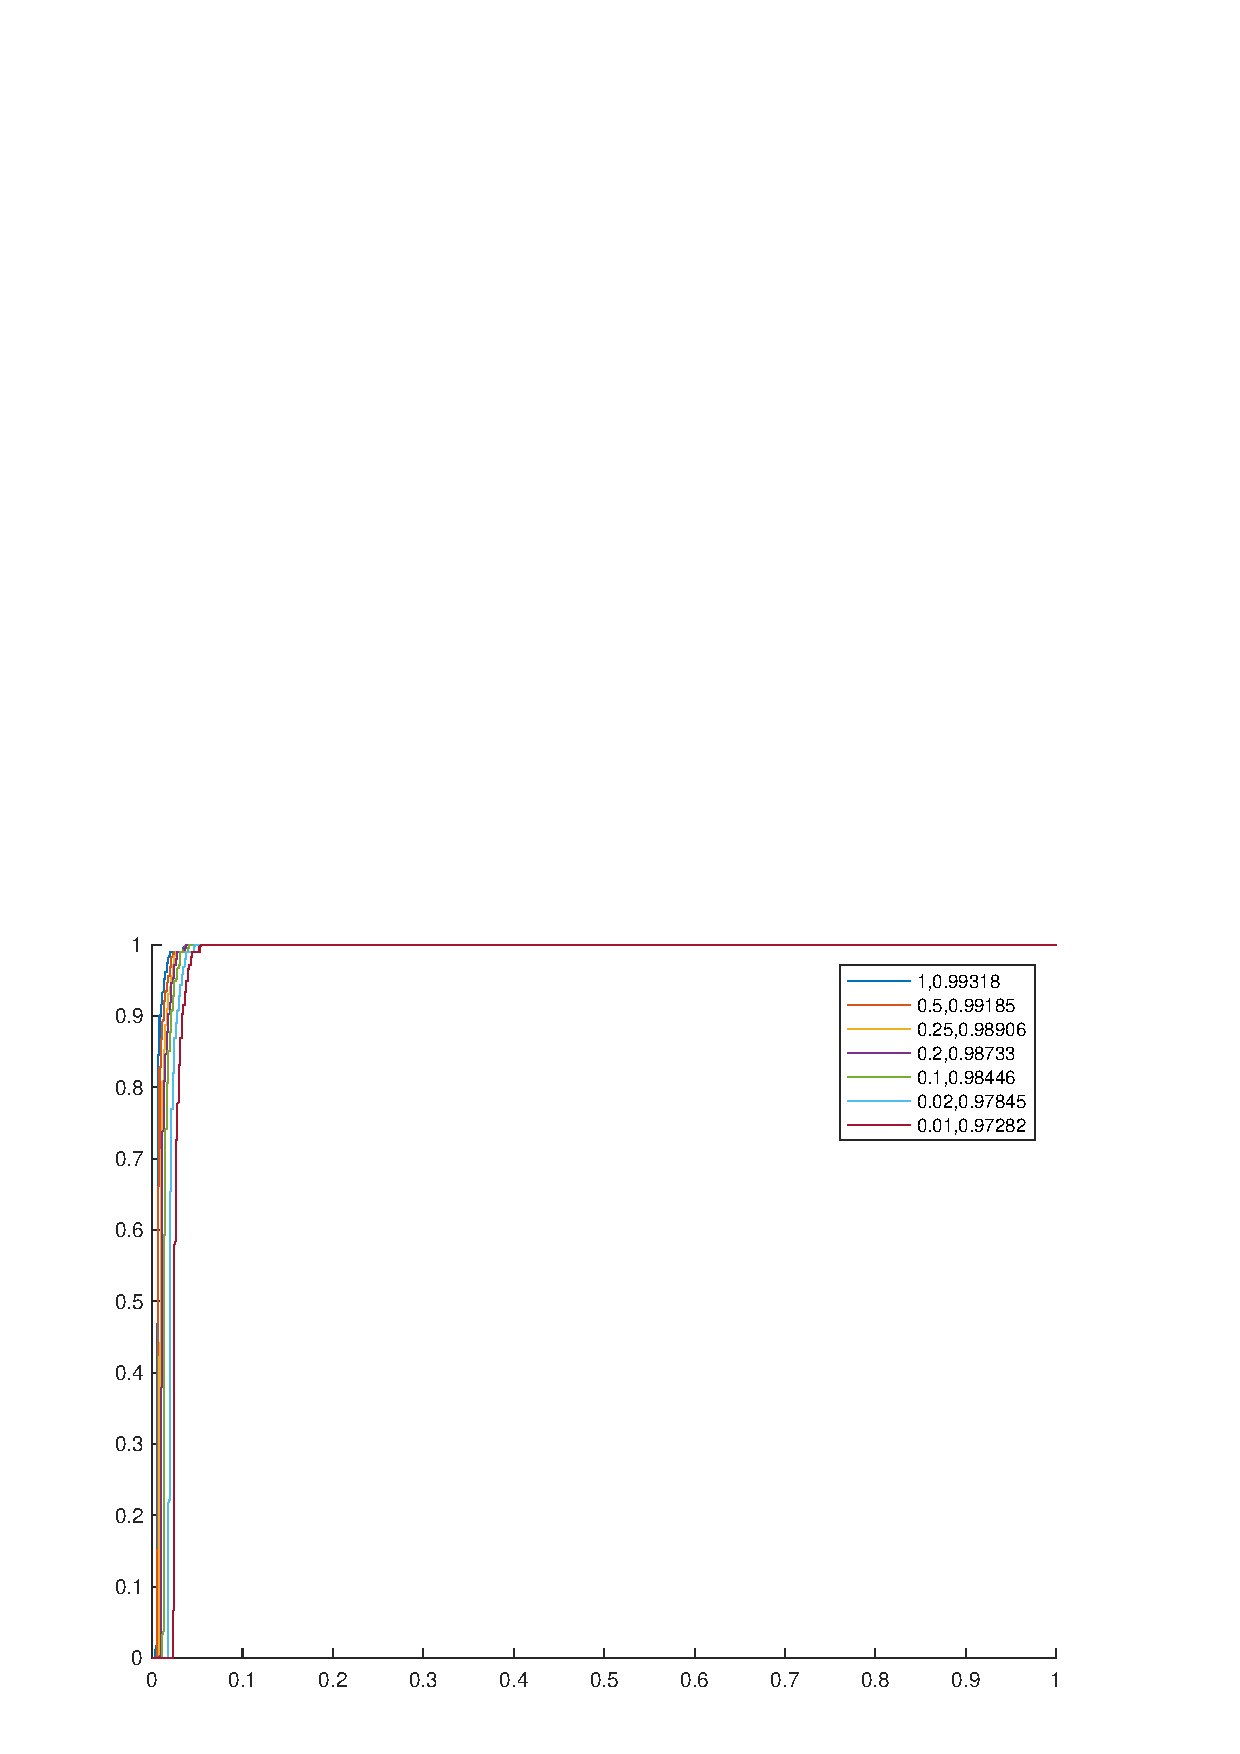
\includegraphics[height = 7.3 cm]{one-shot-different-k.jpg}
\caption{ROC curves for the single-shot algorthm (as outlined in \ref{alg:single-slot}), for a signal in \(\re^{1000}\). The first number in the legend is the ratio \(n/m\), whilst the second is the area under the curve.}
\label{different_k}
\end{figure}


\begin{figure}[h]
\centering
\includegraphics[height = 7.3 cm]{single_shot_snr_-45.jpg}
\caption{ROC curves for the single-shot algorthm (as outlined in \ref{alg:single-slot}), for a signal in \(\re^{1000}\), with noise added at an SNR of \(-4.5\)dB. The first number in the legend is the ratio \(n/m\), whilst the second is the area under the curve.}
\label{different_k}
\end{figure}

\begin{figure}[h]
\centering
\includegraphics[height = 7.3 cm]{single_shot_snr_-105.jpg}
\caption{ROC curves for the single-shot algorthm (as outlined in \ref{alg:single-slot}), for a signal in \(\re^{1000}\), with noise added at an SNR of \(-10.5\)dB. The first number in the legend is the ratio \(n/m\), whilst the second is the area under the curve.}
\label{different_k}
\end{figure}

\begin{figure}[h]
\centering
\includegraphics[height = 7.3 cm]{single_shot_snr_-18.jpg}
\caption{ROC curves for the single-shot algorthm (as outlined in \ref{alg:single-slot}), for a signal in \(\re^{1000}\), with noise added at an SNR of \(-18\)dB. The first number in the legend is the ratio \(n/m\), whilst the second is the area under the curve.}
\label{different_k}
\end{figure}

We now present some results for the multiple-stage algorithm \ref{alg:multiple-shot}.

\begin{figure}[h]
\centering
\includegraphics[height = 7.3 cm]{streaming-no-noise.jpg}
\caption{ROC curves for the multi-shot algorthm (as outlined in \ref{alg:multiple-slot}), for a signal in \(\re^{300}\), over 5 time slots. The first number in the legend is the ratio \(n/m\), whilst the second is the area under the curve. }
\label{different_k}
\end{figure}

In this instance the algorithm is able to provide an estimate, from only two groups i.e. it is able to infer that there is a change in the signal between the 3rd and 4th periods, and use this information to estimate the entire signal. 